%% -----------------------------------------------------------------------------

A type-level mutator is {\em interesting\/} (1) if, upon removal of the type
annotations from the mutant-module, it raises a run-time error, (2) whose stack
trace contains source locations from at least three modules, and (3) if it
applies to all of the to-be-evaluated semantics. The application of an
interesting mutator yields a mutant that represents a {\em debugging scenario\/}
where the rational programmer can exploit blame information.

Let us consider the three conditions in order:
\begin{enumerate}

\item By definition, an impedance mismatch is a class between type ascription of
one module to another module's exports. Hence, the application of a mutator must
create a mutant module that fails to type check. Removing the types from this
module creates an impedance mismatch between it and the modules that import its
services, directly or indirectly. This impedance mismatch is of interest if, and
only if, running the program leads to an exception---otherwise it goes
unobserved and cannot be debugged. 

\item If the evaluation o mutant module immediately raises an exception because
of the mutation, there is no work for the rational programmer. Indeed, if the
stack trace contains source pointers to two modules, the scenario is still
uninteresting. Every ordinary benchmark program comes with a {\tt main} module
that acts as a driver, whose source is guaranteed to be included in the stack
trace.  Hence, the definition of interesting mutator insists on the presence of
three different modules in the stack trace. This guarantees that the debugging
scenario demands a sufficiently sophisticated effort, due to the interaction
between the buggy module with its context.  In these cases, the rational
programmer must examine at least modules to locate the source of the faulty
interaction.

\item The goal of a comparative evaluation is to give the rational programmer a
chance to debug the same scenario using different pieces of information.  In the
case of gradual typing semantics, a meta-theorem due to Greenman and
Felleisen~\cite{gf-icfp-2018} says that if a program raises an exception under
Erasure, it also errors under all other semantics.  Hence, a comparison of blame
information insists that a debugging scenario {\em raises a run-time exception
under Erasure\/}.

{\bf Note} While this choice favors Erasure over Transient and Natural and, for
the same reason, Transient over Natural, some form of bias towards one or the
other semantics is unavoidable. Tipping the scales in favor of the theoretically
weakest semantics yields the most stable results. See
section~\ref{sec:discussion} for some further discussion of this choice.

\end{enumerate}
\mf{It seems to me that we're going out on a limb with this claim. Isn't it true
that the ``three'' is really the result of how many modules are typed/untyped in
the context of the mutant module?}
%
Although the creation of such scenarios depends on both the mutator and the
context of the mutant module, it turns out that some of the discarded mutators 
often generate uninterresting scenarios.


%\begin{figure*}
%  \centering
%  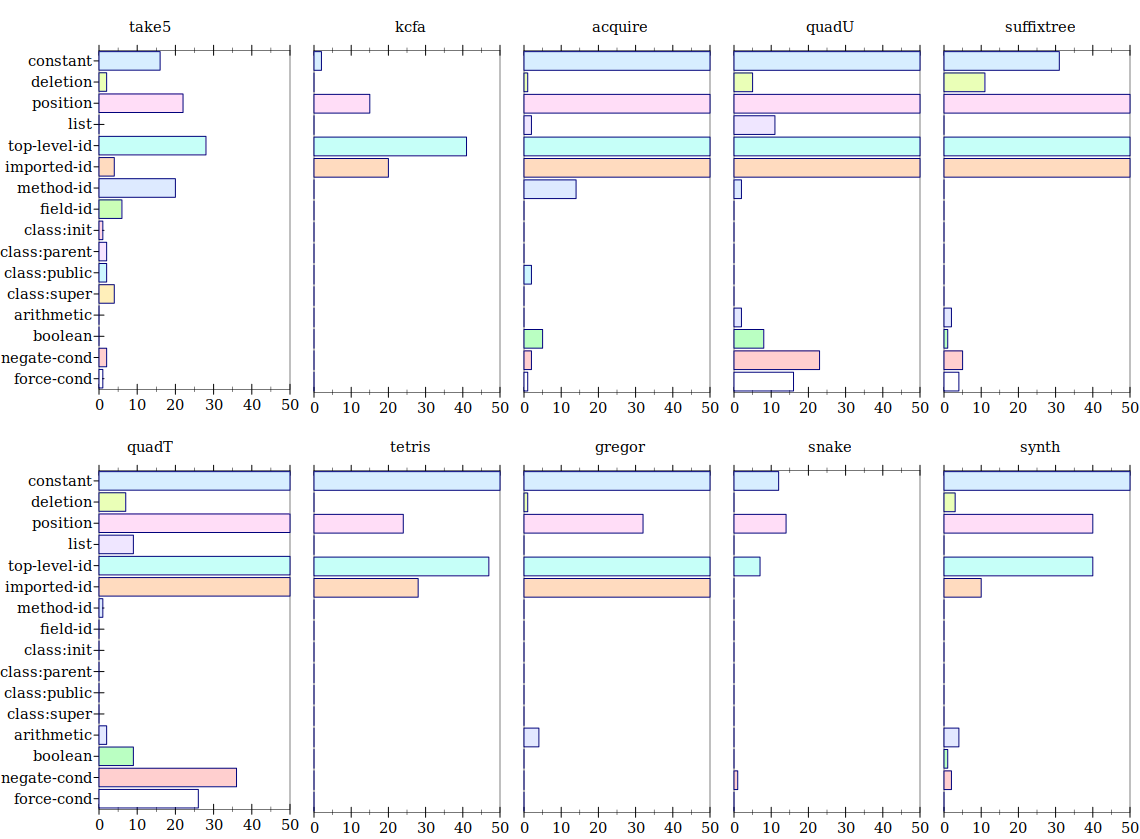
\includegraphics[scale=0.35]{./plots/mutant-breakdown}
%  \caption{Interesting debugging scenarios produced by our mutators. Counts are cut off at 50.}
%  \label{fig:mutant-breakdown}
%\end{figure*}

